\usetikzlibrary{arrows.meta, positioning}

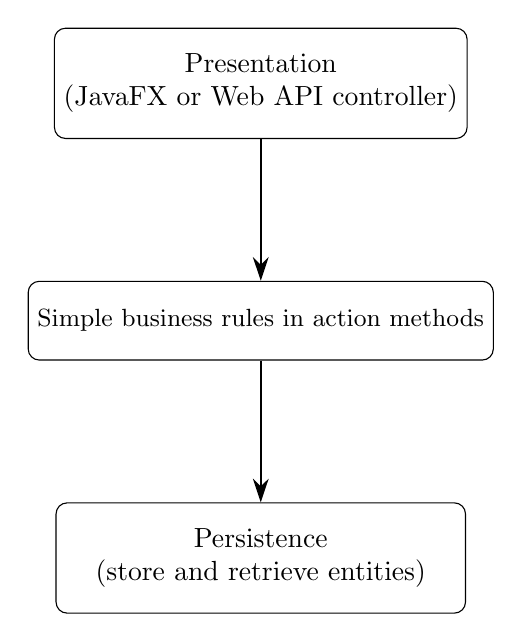
\begin{tikzpicture}[
    node distance=1.8cm and 2.4cm,
    module/.style={draw, rounded corners, minimum width=5.2cm, minimum height=1.4cm, align=center},
    note/.style={draw, rounded corners, minimum width=5.2cm, minimum height=1.0cm, align=center, font=\small},
    dep/.style={-{Stealth[length=3mm, width=2mm]}, thick}
]
    \node[module] (presentation) {Presentation\\(JavaFX or Web API controller)};
    \node[note, below=of presentation] (logic) {Simple business rules in action methods};
    \node[module, below=of logic] (persistence) {Persistence\\(store and retrieve entities)};

    \draw[dep] (presentation.south) -- (logic.north);
    \draw[dep] (logic.south) -- (persistence.north);
\end{tikzpicture}
